\documentclass{article}
\usepackage[utf8]{inputenc}
\usepackage{amsmath}
\usepackage{amssymb}
\usepackage{graphicx}

\begin{document}

\section*{Solving a quasi-linear system}
We consider the \textit{nonlinear} (quasi-linear) system
\begin{equation}
    \mathbf{A}\left(\mathbf{x}\right)\mathbf{x} = \mathbf{b}
\end{equation}
The function $A : \mathbb{R}^{n} \to \mathbb{R}^{n,n}$ is a matrix-valued function
\begin{equation*}
    \mathbf{A}\left(\mathbf{x}\right) := \begin{bmatrix}
        \gamma\left(\mathbf{x}\right) & 1 & & &  \\
        1 & \gamma\left(\mathbf{x}\right) & 1 &&\\
        & \ddots & \ddots & \ddots && \\
        &&\ddots & \ddots & \ddots & \\
        &&& 1 & \gamma\left(\mathbf{x}\right) & 1 \\
        &&&& 1 & \gamma\left(\mathbf{x}\right) 
    \end{bmatrix} \: \text{,} \quad \gamma\left(\mathbf{x}\right) := 3 + \left\lVert \mathbf{x}\right\rVert_{2}
\end{equation*}
and  $\left\lVert\:.\:\right\rVert_{2}$ is the Euclidean norm.
\subsection*{8-10.a} 
We want to observe how we get from $ \mathbf{A}\left(\mathbf{x}^{\left(k\right)}\right)$ to $ \mathbf{A}\left(\mathbf{x}^{\left(k+1\right)}\right)$, the task description tells us that we take the argument to the matrix valued function from the \textbf{previous} step and just solve a linear system for the \textbf{next} iterate. Putting this into the equation (1) we get
\begin{equation*}
    \mathbf{A}\left(\mathbf{x}^{\left(k\right)}\right)\mathbf{x}^{\left(k+1\right)} = \mathbf{b} \Longleftrightarrow \mathbf{x}^{\left(k+1\right)} = \mathbf{A}\left(\mathbf{x}^{\left(k\right)}\right)^{-1}\mathbf{b}
\end{equation*}
\subsection*{8-10.b}
The wording "efficient" and the structure of the matrix $\mathbf{A}$ do already imply that we can compute both the inverse and the matrix-vector product needed more efficiently. We know that $\mathbf{A}$ is tridiagonal, we have seen qr-decomposition based efficient solving of a system $Ax = b$, however the task taking 10 minutes and the hint suggest that a somewhat naive approach may be enough. We need to use sparse matrix types and hence the \textbf{reserve} functionality to "allocate" space in our matrix, this can be done by seeing that we need a bit less than three times the diagonal which has the size of the length of the input vector \textit{xk}. A google search actually shows us that the Eigen documentation sometimes contains somewhat useful information (https://eigen.tuxfamily.org/dox/group\_\_TutorialSparse.html), the method \textit{A.insert(row, col) = value} allows us to set values in the sparse matrix. We can then finally solve the system using the 
\begin{equation*}
  \text{Eigen::SparseLU}<\text{Eigen::SparseMatrix}<\text{double}>>  
\end{equation*}
functionality which behaves like the general LU decomposition.

\pagebreak

This produces the following code

\begin{figure}[!hbt]
    \centering
    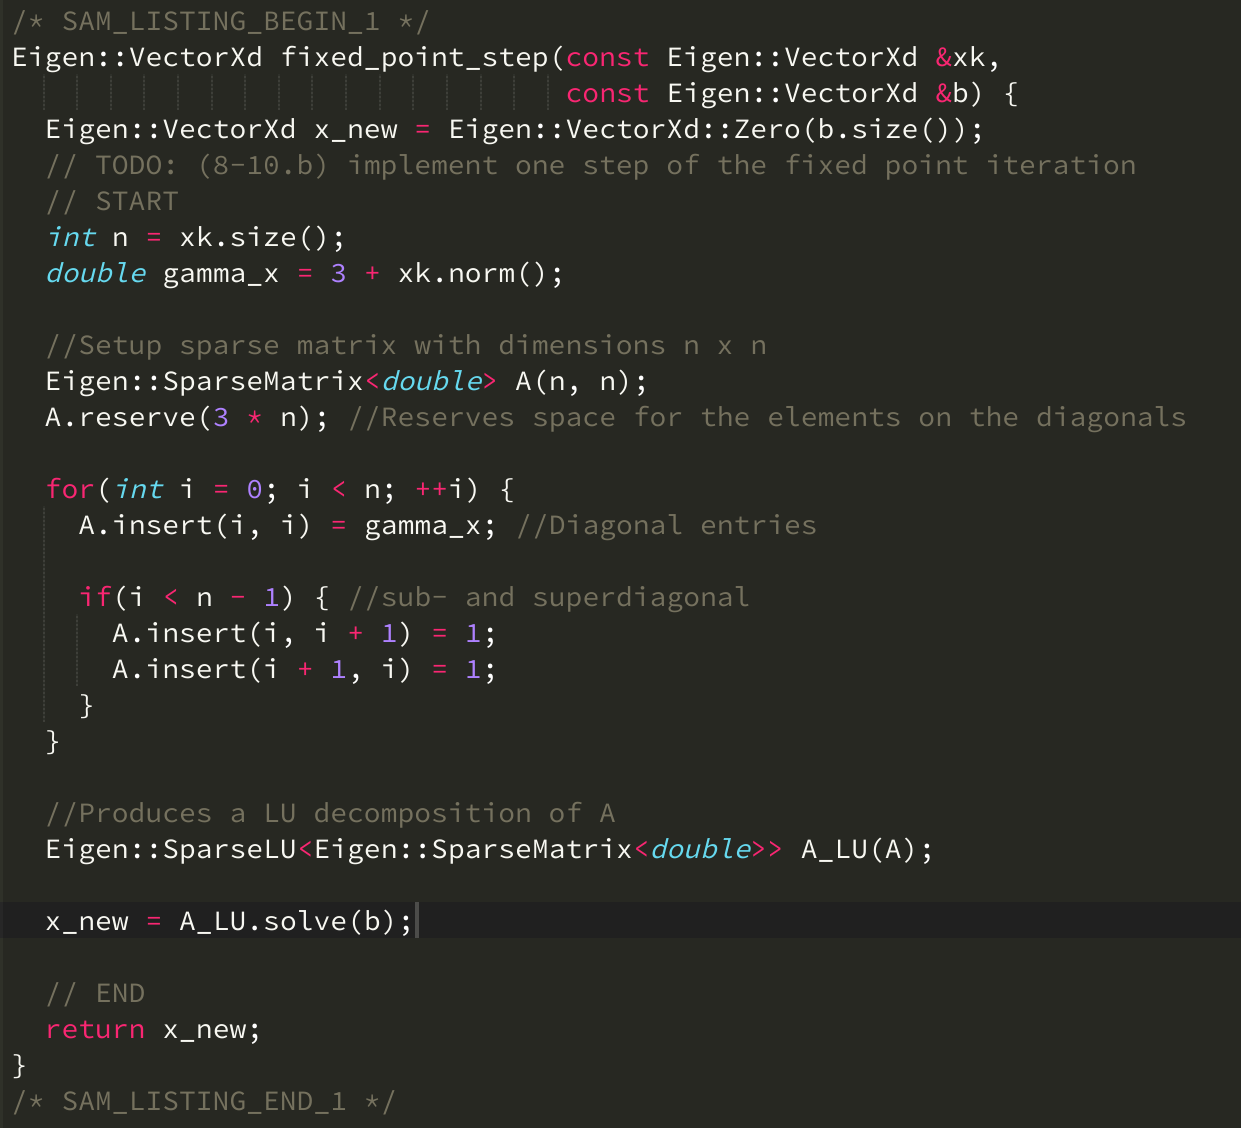
\includegraphics[width=0.8\linewidth]{FixedPointIt8_10.png}
\end{figure}

\subsection*{8-10.c}
We are now tasked with using the fixed-point iteration found before with $\mathbf{x}^{\left(0\right)} = \mathbf{b}$ as an initial guess. We should use a correction based stopping criterion. Let us first look at this criterion. The lecture document on page 594 describes said criterion as follows

\begin{figure}[!hbt]
    \centering
    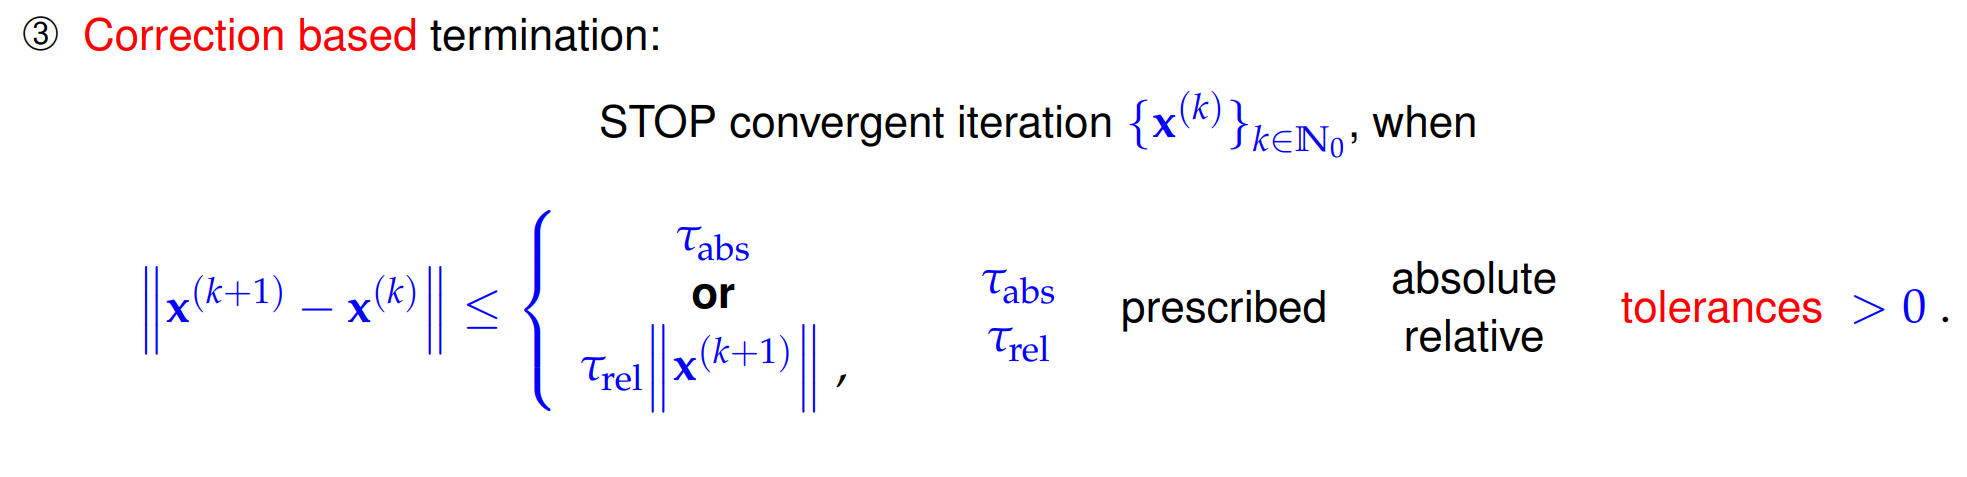
\includegraphics[width=0.9\linewidth]{CorrectionBasedCriterion.png}
\end{figure}


\noindent This gives us the idea for our termination criterion implementation, we can put this into a while loop and iterate until we are happy with the result. 

\pagebreak

This produces the following code
\begin{figure}[!hbt]
    \centering
    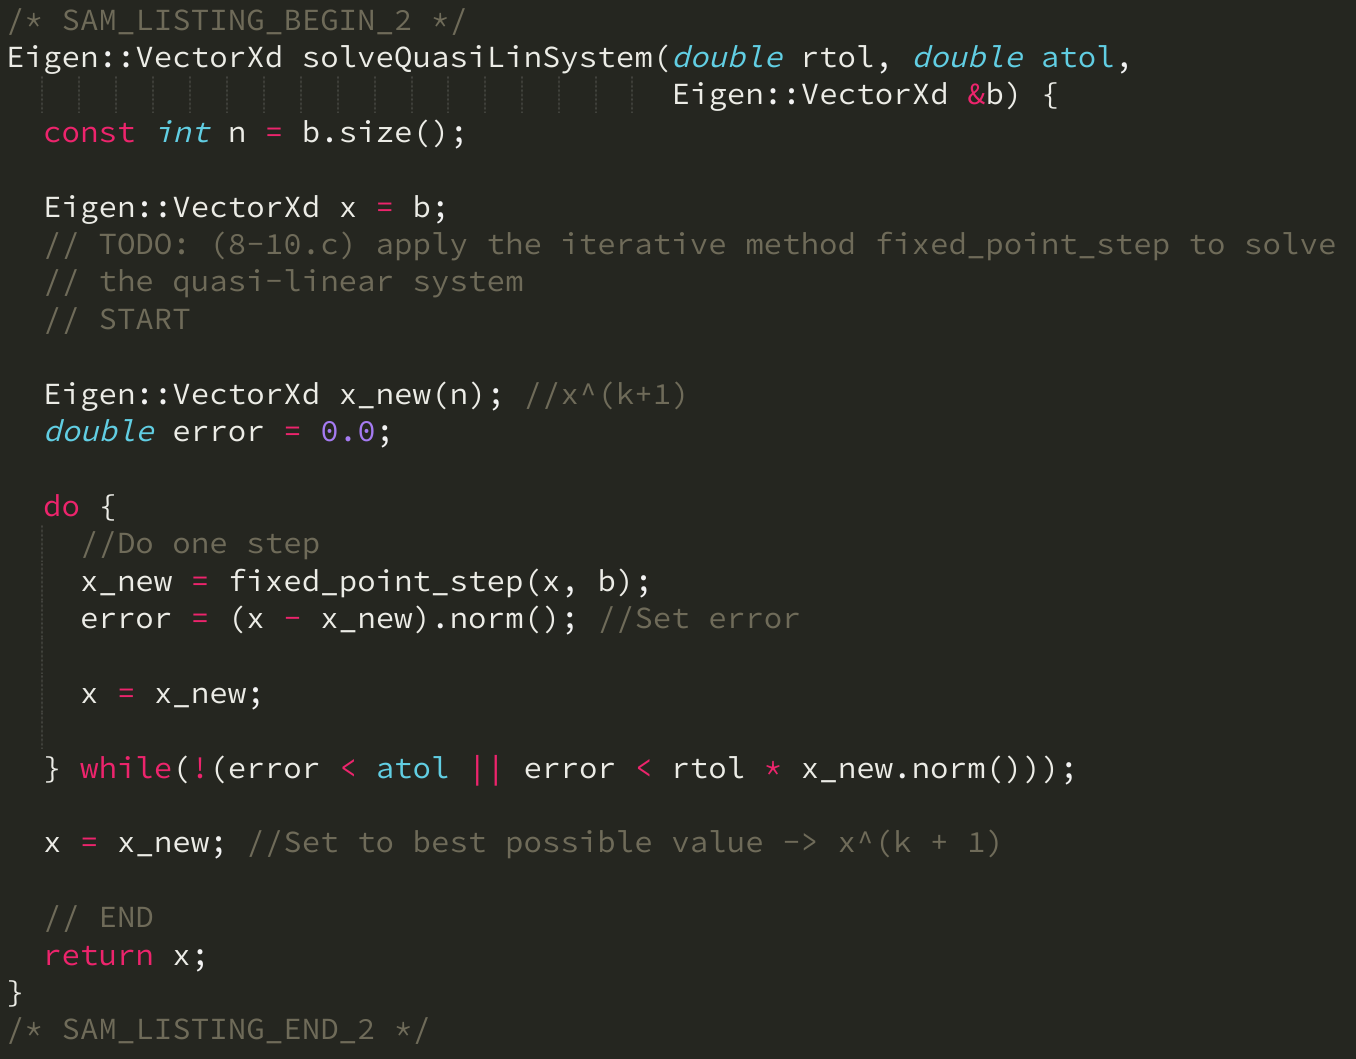
\includegraphics[width=0.9\linewidth]{8_10b.png}
\end{figure}

\subsection*{8-10.d} 
To solve $\mathbf{A}\left(\mathbf{x}\right)\mathbf{x} = \mathbf{b}$ using the Newton's method we have to solve
\begin{equation*}
    \mathbf{A}\left(\mathbf{x}\right)\mathbf{x} - \mathbf{b} = 0
\end{equation*} We will now use the derivation of example 8.5.1.30 to get the Newton iteration. We first use the matrix $\mathbf{T}$ given to us by
\begin{equation*}
    \mathbf{T} = \begin{bmatrix}
        3 & 1 & & &  \\
        1 & 3 & 1 &&\\
        & \ddots & \ddots & \ddots && \\
        &&\ddots & \ddots & \ddots & \\
        &&& 1 & 3 & 1 \\
        &&&& 1 & 3 
    \end{bmatrix}
\end{equation*}
to rewrite the given system (1) to
\begin{equation*}
    \mathbf{A}\left(\mathbf{x}\right)\mathbf{x} = \mathbf{T}\mathbf{x} + \mathbf{x}\left\lVert \mathbf{x} \right\rVert_{2}
\end{equation*}
We need to take a look at the discussion following Def. 8.5.1.13. now. This section talks about the derivative of an Euclidean norm. The concept of "High level differentiation" is introduced. Given a function $F\left(\mathbf{x}\right) := \left\lVert \mathbf{x}\right\rVert$ we can write $F$ as a composition of two functions $F = G \circ H$ 
\begin{equation*}
    G\left(\xi\right) := \sqrt{\xi} \quad H\left(\mathbf{x}\right) := \mathbf{x}^{\mathsf{T}}\mathbf{x}
\end{equation*}
We can apply the rule for differentiation of a bilinear form
\begin{equation*}
    \mathrm{D}\Psi\left(\mathbf{x}\right) \mathbf{h} = \underbrace{\left(\mathbf{x}^{\mathsf{T}}\mathbf{A}^{\mathsf{T}} + \mathbf{x}^{\mathsf{T}\mathbf{A}}\right)\mathbf{h}}_{=\left(\text{\textbf{grad}}\left(\Psi\left(\mathbf{x}\right)\right)\right)^{\mathsf{T}}}
\end{equation*}
seen on Example 8.5.1.19. we get
\begin{equation*}
    \mathrm{D}H\left(\mathbf{x}\right)\mathbf{h} = 2\mathbf{x}^{\mathsf{T}}\mathbf{h} \quad \mathrm{D}G\left(\xi\right)\xi = \frac{\xi}{2\sqrt{\xi}}
\end{equation*}
Applying the chain rule then gives us
\begin{equation*}
    \mathrm{D}F\left(\mathbf{x}\right)\mathbf{h} = \mathrm{D}G\left(H\left(\mathbf{x}\right)\mathbf{h}\right)\left(\mathrm{D}H\left(\mathbf{x}\right)\mathbf{h}\right) = \frac{2\mathbf{x}^{\mathsf{T}}\mathbf{h}}{2 \sqrt{\mathbf{x}^{\mathsf{T}}\mathbf{x}}} = \frac{\mathbf{x}^{\mathsf{T}}}{\left\lVert \mathbf{x} \right\rVert_{2}}\cdot \mathbf{h}
\end{equation*}
Hence using definition 8.5.1.18 we can see that 
\begin{equation*}
    \text{\textbf{grad}}\left(F\left(\mathbf{x}\right)\right) = \frac{\mathbf{x}}{\left\lVert \mathbf{x} \right\rVert_{2}}
\end{equation*}
The same result can be achieved by simply writing down the norm via its components and then looking at the partial derivatives and seeing the same result (I prefer this). We can hence now do the derivation
\begin{equation*}
    \mathrm{D}F\left(\mathbf{x}\right)\mathbf{h} = \mathbf{T}\mathbf{h} + \left\lVert \mathbf{x} \right\rVert_{2}\mathbf{h} + \mathbf{x}\frac{\mathbf{x}^{\mathsf{T}}\mathbf{h}}{\left\lVert \mathbf{x} \right\rVert_{2}} = \left(\mathbf{A}\left(\mathbf{x}\right) + \frac{\mathbf{x}\mathbf{x}^{\mathsf{T}}}{\left\lVert \mathbf{x} \right\rVert_{2}} \right) \mathbf{h}
\end{equation*}
Hence the Newton Iteration defined by
\begin{equation*}
    \mathbf{x}^{\left(k+1\right)} = \mathbf{x}^{\left(k\right)} - \frac{F\left(\mathbf{x}^{\left(k\right)}\right)}{F'\left(\mathbf{x}^{\left(k\right)}\right)}
\end{equation*}
is written as
\begin{equation*}
    \mathbf{x}^{\left(k+1\right)} = \mathbf{x}^{\left(k\right)} - \left(\mathbf{A}\left(\mathbf{x}^{\left(k+1\right)}\right) + \frac{\mathbf{x}^{\left(k\right)}\left(\mathbf{x}^{\left(k\right)}\right)^{\mathsf{T}}}{\left\lVert \mathbf{x}^{\left(k\right)} \right\rVert_{2}} \right)^{-1}\left(\mathbf{A}\left(\mathbf{x}^{\left(k\right)}\right)\mathbf{x}^{\left(k\right)} - \mathbf{b}\right)
\end{equation*}
The inversion is the "analog" operation to division for number but for matrices.
\subsubsection*{8-10.e}
The Sherman-Morrison-Woodbury update formula for rank-one modifications and $\mathbb{K} = \mathbb{R}$ is given by (Remark 8.6.0.14 shows a similar derivation which could be useful in an exam)
\begin{equation*}
    \left(\mathbf{A} + \mathbf{u}\mathbf{v}^{\mathsf{T}}\right)^{-1} = \left(\mathbf{I} - \frac{\mathbf{A}^{-1}\mathbf{u}\mathbf{v}^{\mathsf{T}}}{1 + \mathbf{v}^{\mathsf{T}}\mathbf{A}^{-1}\mathbf{u}}\right)\mathbf{A}^{-1} \quad \text{for} \quad 1 + \mathbf{v}^{\mathsf{T}}\mathbf{A}^{-1}\mathbf{u} \neq 0
\end{equation*}

\pagebreak 

\noindent A horrendous and error-prone derivation would then give us the result, this is a bit to tedious, so here the derivation on its own:
\begin{figure}[!hbt]
    \centering
    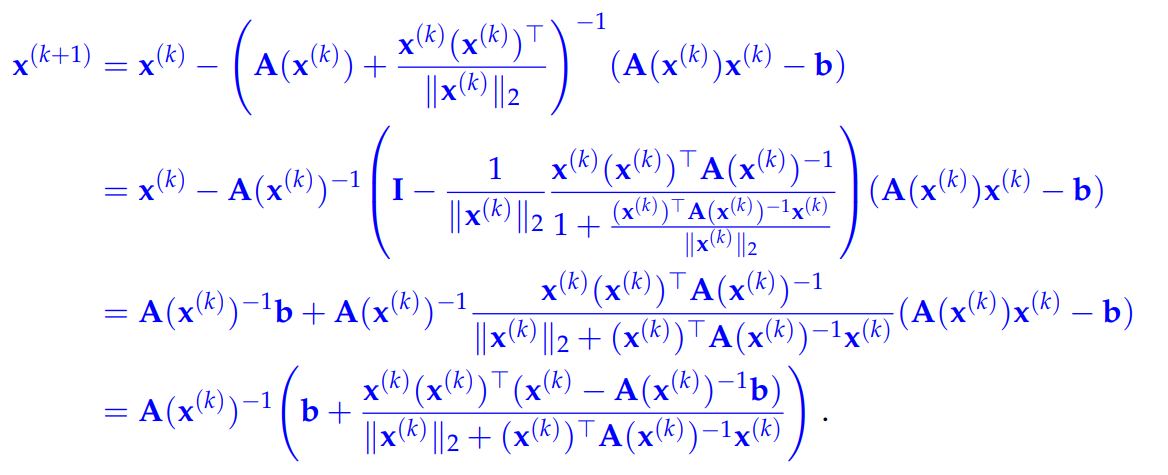
\includegraphics[width=0.9\linewidth]{DerivationSMW.png}
\end{figure}

\pagebreak

\subsection*{8.10-f} 
We use a similar approach as in 8-10.b and modify the formula above a bit to get
\begin{equation*}
    \mathbf{x}^{\left(k+1\right)} = \mathbf{A}\left(\mathbf{x}^{\left(k\right)}\right)^{-1}\mathbf{b} + \mathbf{A}\left(\mathbf{x}^{\left(k\right)}\right)^{-1}\left(\mathbf{x}\right)^{\left(k\right)} \cdot \frac{\left(\mathbf{x}^{\left(k\right)}\right)^{\mathsf{T}} \cdot \left(\mathbf{x}^{\left(k\right)} - \mathbf{A}\left(\mathbf{x}^{\left(k\right)}\right)^{-1}\mathbf{b}\right)}{\left\lVert \mathbf{x}^{\left(k\right)} \right\rVert_{2} + \left(\mathbf{x}^{\left(k\right)}\right)^{\mathsf{T}}\mathbf{A}\left(\mathbf{x}^{\left(k\right)}\right)^{-1} \mathbf{x}^{\left(k\right)}}
\end{equation*}
We have the two following systems we can solve using a single LU-decomposition
\begin{equation*}
\mathbf{A}\left(\mathbf{x}^{\left(k\right)}\right)^{-1}\mathbf{b} = \mathbf{x}_{1} \quad \text{,} \quad \mathbf{A}\left(\mathbf{x}^{\left(k\right)}\right)^{-1}\mathbf{x}^{\left(k\right)} = \mathbf{x}_{2}
\end{equation*}
where $x_{1}$ is \textit{Abx} and $x_{2}$ is \textit{Axx} in the code below.

\begin{figure}[!hbt]
    \centering
    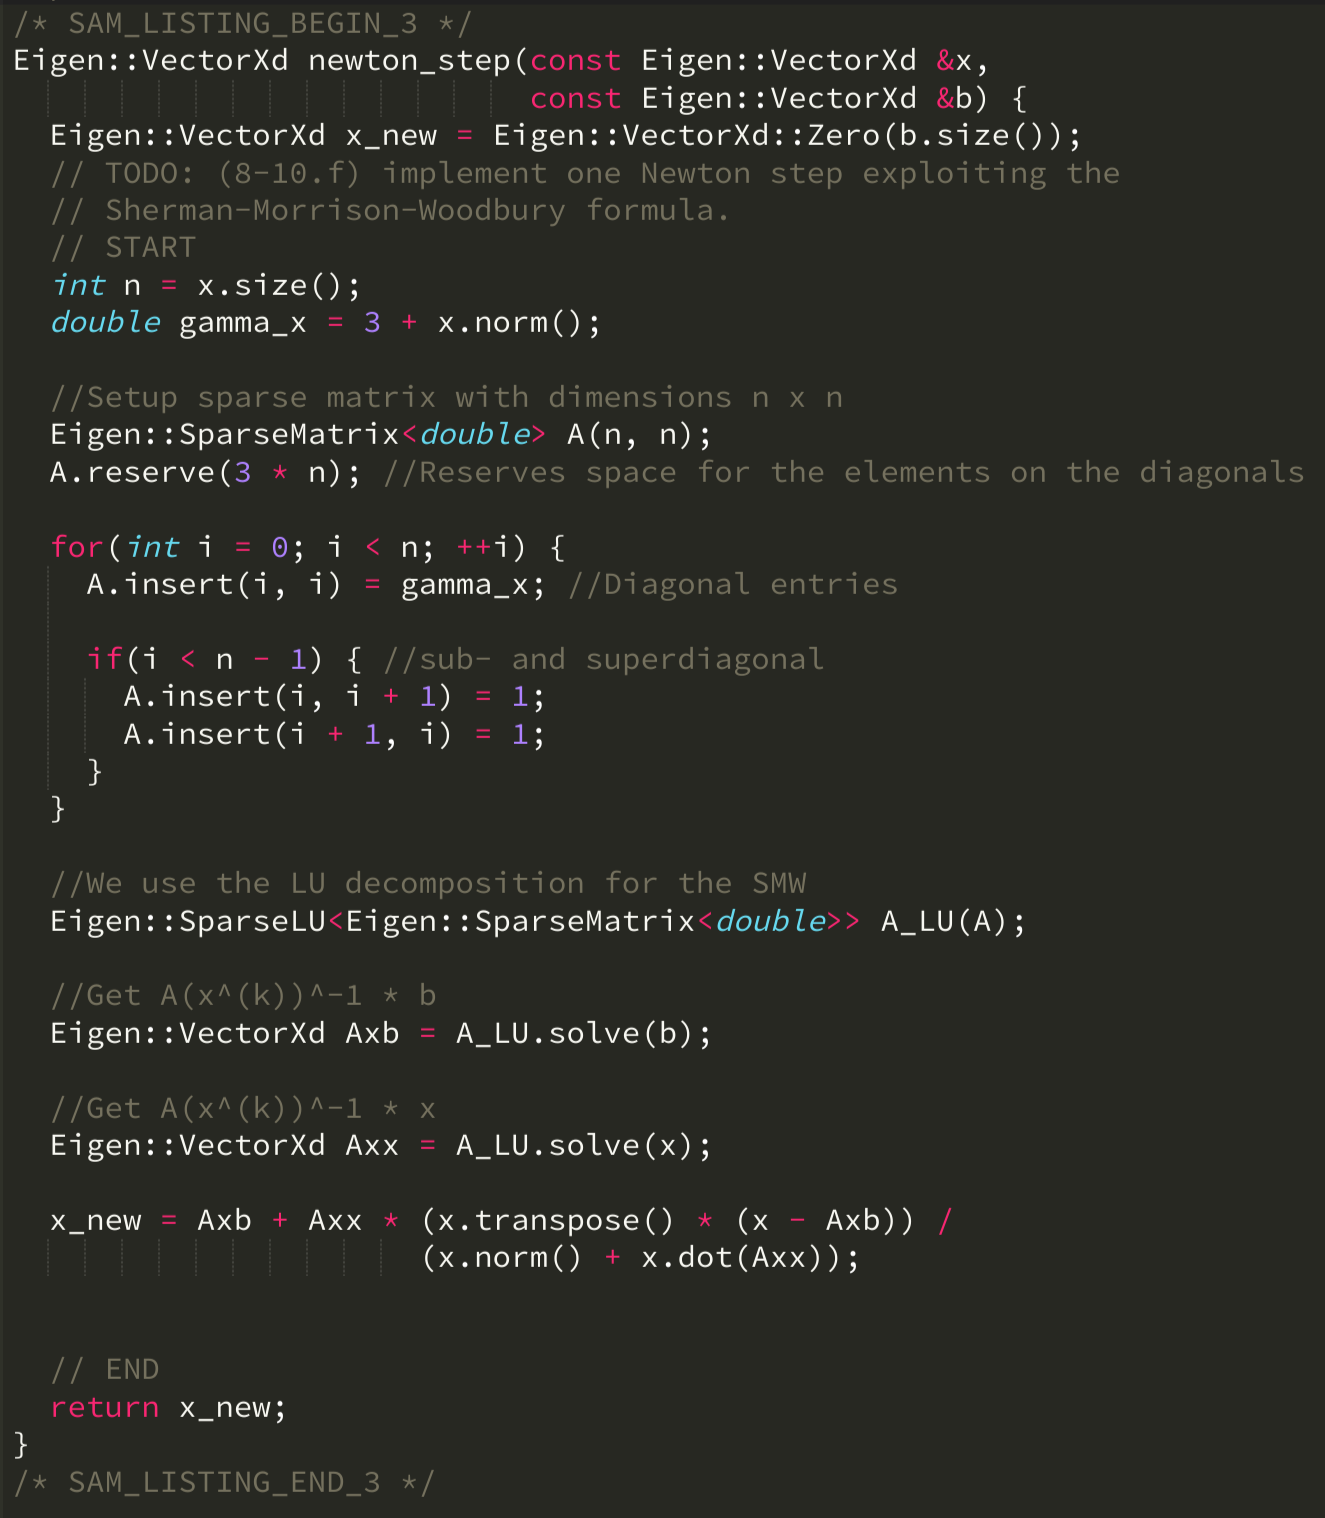
\includegraphics[width=0.9\linewidth]{8-10.f.png}
\end{figure}
\subsection*{8-10.g}
We use the almost identical code as in 8-10.c again, this results in the code below:

\begin{figure}[!hbt]
    \centering
    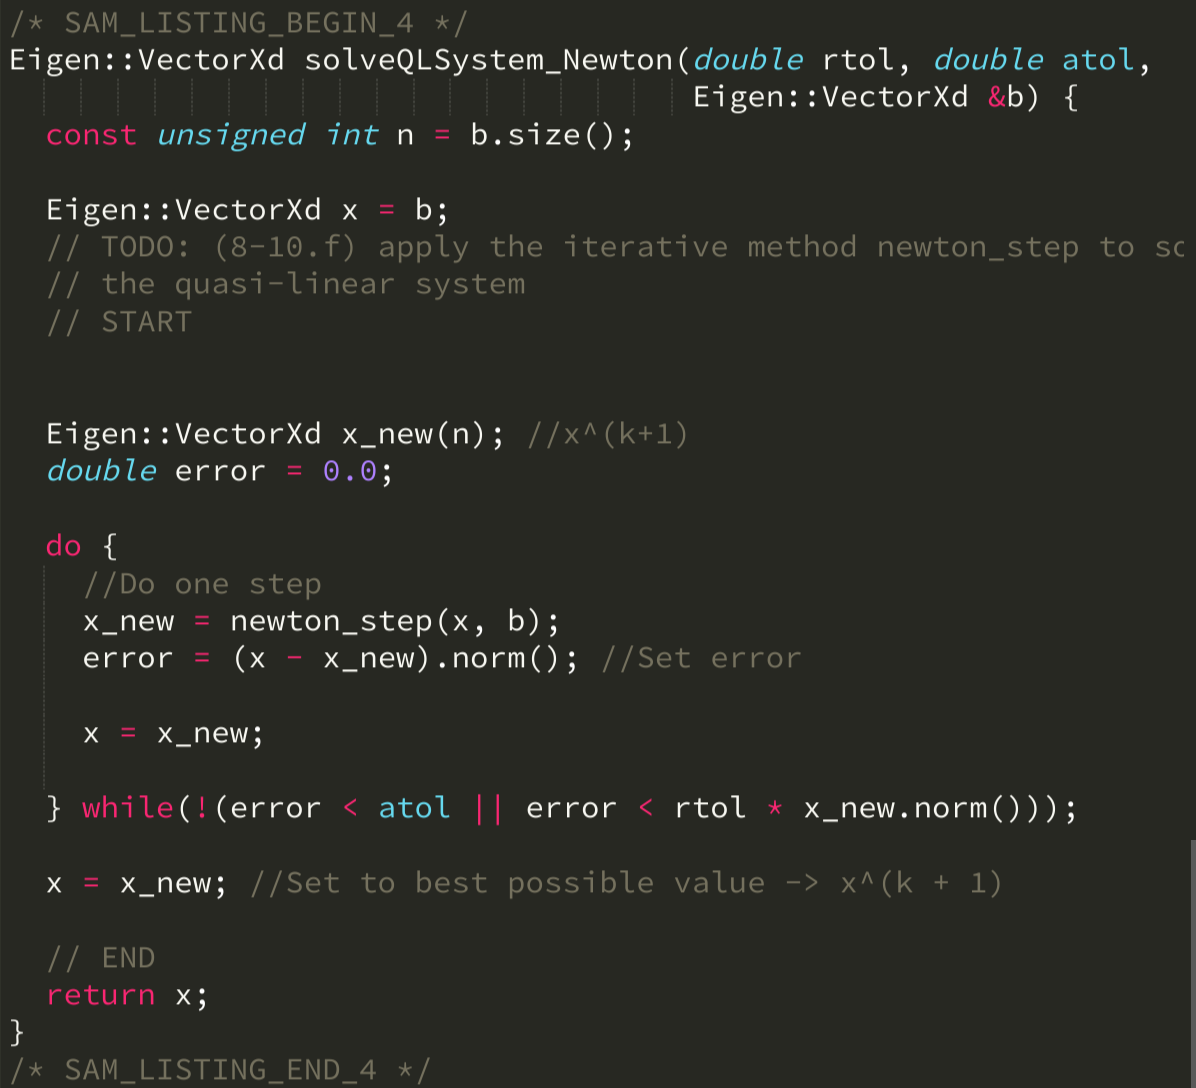
\includegraphics[width=0.9\linewidth]{8-10.g.png}
\end{figure}
\end{document}
